% Capstone Final Project Report
% Spring 2014
% Val Red, Eric Cuiffo, Jeff Adler, Parth Desai, Jeff Rabinowitz
% All rights reserved.

\documentclass[12pt,letterpaper,titlepage]{report}


\usepackage[margin=1in]{geometry}

\usepackage{amsmath}
%\bibliographystyle{ieeetr}
\usepackage{graphicx}
\usepackage{subfig}
\usepackage{titling}
\usepackage{fontspec}
%\usepackage[utf8]{inputenc}
\usepackage{csquotes}
\usepackage[style=ieee,backend=biber,bibencoding=utf8]{biblatex}
	\addbibresource{citations.bib}
%\usepackage{biblatex-ieee}
%\usepacakge{multicol}
\usepackage[bookmarks=true]{hyperref}
\hypersetup{
    %bookmarks=false,    % show bookmarks bar?
    pdftitle={},    % title
    pdfauthor={},                     % author
    pdfsubject={},        % subject of the document
    pdfkeywords={}, % list of keywords
    colorlinks=true,       % false: boxed links; true: colored links
    linkcolor=blue,       % color of internal links
    citecolor=black,       % color of links to bibliography
    filecolor=black,        % color of file links
    urlcolor=blue,        % color of external links
    linktoc=page            % only page is linked
}%

\usepackage{abbrevs}
\usepackage{minted}

\setsansfont{Calibri}
\setmonofont{Consolas}
\renewcommand{\theFancyVerbLine}{
  \sffamily\textcolor[rgb]{0.5,0.5,0.5}{\scriptsize\arabic{FancyVerbLine}}}

\begin{document}
% This inserts the Title, Author, and Date here.
%\maketitle
\begin{titlepage}

\newcommand{\HRule}{\rule{\linewidth}{0.5mm}} % Defines a new command for the horizontal lines, change thickness here


\center % Center everything on the page
 
%----------------------------------------------------------------------------------------
%	HEADING SECTIONS
%----------------------------------------------------------------------------------------

\textsc{\LARGE Rutgers University}\\[1.5cm] % Name of your university/college
\textsc{\Large Capstone Senior Design Project}\\[0.5cm] % Major heading such as course name
\textsc{\large 14:332:492}\\[1.0cm] % Minor heading such as course title

%----------------------------------------------------------------------------------------
%	TITLE SECTION
%----------------------------------------------------------------------------------------

\HRule \\[0.4cm]
{ \huge \bfseries Scarletshield}\\
  \Large A Lightweight, Linux-based Network Security Solution Suite \\[0.4cm] % Title of your document
\HRule \\[3.5cm]
 
%----------------------------------------------------------------------------------------
%	AUTHOR SECTION
%----------------------------------------------------------------------------------------

\begin{minipage}{0.4\textwidth}
\begin{flushleft} \large
\emph{Team:}\\
Jeff \textsc{Adler}\\ % Your name
Eric \textsc{Cuiffo}\\
Parth \textsc{Desai}\\
Jeff \textsc{Rabinowitz}\\
Val A. \textsc{Red}
\end{flushleft}
\end{minipage}
~
\begin{minipage}{0.4\textwidth}
\begin{flushright} \large
\emph{Advisor:} \\
Dr. Manish \textsc{Parashar} % Supervisor's Name
\end{flushright}
\end{minipage}\\[4cm]

% If you don't want a supervisor, uncomment the two lines below and remove the section above
%\Large \emph{Author:}\\
%John \textsc{Smith}\\[3cm] % Your name

%----------------------------------------------------------------------------------------
%	DATE SECTION
%----------------------------------------------------------------------------------------

{\large \today}\\[3cm] % Date, change the \today to a set date if you want to be precise

%----------------------------------------------------------------------------------------
%	LOGO SECTION
%----------------------------------------------------------------------------------------

%\includegraphics{Logo}\\[1cm] % Include a department/university logo - this will require the graphicx package
 
%----------------------------------------------------------------------------------------

\vfill % Fill the rest of the page with whitespace

\end{titlepage}


\tableofcontents
\pagebreak


\newabbrev{\scarletshield}{``Scarletshield''}[Scarletshield]

\newabbrev{\dos}{Denial-of-service (DoS)}[DoS]
\newabbrev{\ddos}{Distributed Denial-of-service (DDoS)}[DDoS]
\newabbrev{\apt}{Advanced Persistent Threat (APT)}[APT]
\newabbrev{\did}{Defense in Depth (DiD)}[DiD]
\newabbrev{\nsa}{National Security Agency (NSA)}[NSA]
\newabbrev{\dns}{Domain Name Service (DNS)}[DNS]
\newabbrev{\ctwo}{Command-and-control (C2)}[C2]
\newabbrev{\distros}{distributions (distros)}[distros]

{
\setlength{\parskip}{1em}
\chapter{Abstract}

\scarletshield is a customized Ubuntu 12.04 LTS image featuring a uniquely
layered cyber security deployment of several open source services; most notably
the \textbf{''Snort'' Intrusion Detection System (IDS)} utilizing packet inspection and the
\textbf{''Fail2ban'' Intrusion Prevention System (IPS)} utilizing log inspection.  It is
optimized for synergetic network defense and complemented by a dynamic, modern
web frontend providing the utmost flexibility for network administrators to
monitor and quickly react to any and all threats against a network.  The design
of  was conceived as a proof-of-concept to expand upon the more
orthodox but aging \did strategy that layers \emph{overlapping}
technologies rather than presenting varied layers of \emph{complement} defense services
working in \emph{synergy}, which is the approach use to expand upon the defense-in-
depth strategy.  In addition, \scarletshield enables the potential for a user to
interface with interconnected subnets and gateways over a private network to
enable scalability and mitigate large-scale attacks.  Overall, \scarletshield is
intended to be a flexible, open-source system for preventing and thwarting
evolving \ddos Attacks and \apt
by implementing a synergy of various open source and custom
designed services designed to be as flexible and as intuitive as possible for
the network administrator to interface with, minimizing administrative overhead
and maximizing mobility for the network administrator to track and react to
threats.

\section{Introduction}

Attackers have the edge in the dynamically evolving field of cyber security.
With a wider breadth of strategies, near-infinite resources, and a virtually
untraceable mask of anonymity; hackers have long boasted the advantage,
successfully rendering useless the generally accepted \did layered
defense mechanisms most organizations deployed for network defense.
Essentially, is analogous to an onion: although it is deeply
layered, it can be peeled.  Utilizing an even wider breadth of tools and
resources, hackers have successfully and continuously developed new and advanced
approaches, exploits, \dos methods, etc. to employ a
persistent, peeling threat designed to break down or even bypass the \did 
approach employed by network administrators.  In essence, this summarizes
the \apt, which is not a single exploit/attack or even a
collection of exploits/attacks: APT is a \emph{campaign} involving possibly several of
different collections of exploits and attack methodologies and even multiple
actors across different machines that may exist in different countries.

\didlong \autocite{nsa}, as described by the \nsa, is
“[a] practical strategy for achieving Information Assurance in today's highly
networked environments.  It is a ``best practices'' strategy in that it relies on
the intelligent application of techniques and technologies that exist today.”

While \did appears sound in its introduction, a closer and modern
interpretation of later details in the \nsa strategy employing defense-in-depth
shows some of its flaws that come with age, for example: ``To effectively resist
attacks [...] an organization needs to \emph{characterize its adversaries}, their
potential motivations, and their \emph{classes of attack}.''

\begin{figure}[h!]
	\centering
  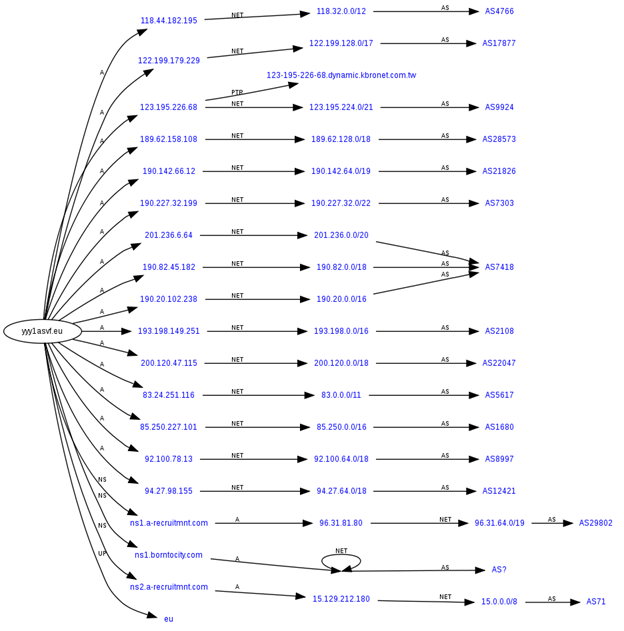
\includegraphics[height=12cm]{./fastflux.png}
  \caption{A visualization of the domain fast-flux. Note the large
  number of IP addresses and domains mapping to a single fully qualified
  domain name used for the C2 server.}
\end{figure}

The above notion presented by the \nsa is idealistic at best in today's climate
of virtually untraceable, anonymous hackers employing robust \dns
techniques such as \textbf{fast flux} \autocite{honey}, which essentially accomplishes hiding a
single \ctwo server by utilizing numerous IP addresses and a
single, rotatable (in an even more difficult-to-trace \textbf{double-flux} methodology)
fully qualified domain name (something as simple as valred.com or hackr.ru, for
example) to very quickly swap between the available IP addresses and \dns records
to avoid detection and backtracing.  Thanks to these particular methods,
problems such as phishing will be omnipresent in the foreseeable future,
exasperated by other countries boasting lax restrictions with regulating the
domain name provisioning.  As such, the NSA’s notion of having organizations
``characterize its adversaries,'' is among the highly impractical and dated points
that weaken the argument for the defense-in-depth strategy.  The only likely
moment adversaries are to be characterized is when it is too late and a network
has already been compromised, such as when the Syrian Electronic Army (SEA)
successfully executed a man-in-the-middle attack rerouting traffic to the U.S.
Marines \autocite{syrians} in 2013.  As such, we keep \scarletshield lightweight and practical
by not addressing this issue; instead, we specifically handle threat prevention
and detection.

Strengths of the defense-in-depth methodology are applied in the implementation
of \scarletshield.  Particularly, one directed focus is on protecting the most
exposed web-facing systems that are typically the target of automated attacks.
This is specifically handled by the robustness of the Snort IDS, which
essentially sniffs all types of Internet Protocol (IP) packets (TCP, UDP, ICMP,
etc.), and checks against patterns, or \emph{rules} and \emph{signatures} indicative of an
attack.  This is reinforced even further by the log-inspection capabilities of
fail2ban, which can essentially pattern-match very common exploits and \dos
traces against typical protocols such as HTTP, SSH
(Secure SHell, which we utilize to remotely access and work on the Scarletshield server)
, and FTP 
(File Transfer Protocol, commonly used for storing and transferring files from a remote server)
and react by
blocking IP addresses logged via ``iptables'', a powerful firewall built into most
modern Linux \distros.

Even though iptables comes with modern Linux \distros by default, many end users
beyond actual system and network administrators fail to utilize iptables to its
full potential.  \scarletshield can partly fill the role for a network
administrator when an end user does not have the personnel or resources to fully
utilize iptables themselves.  It can essentially be connected to any switch or
router and be configured to act as a network gateway such that all traffic to
any end user on a network will have to make it past \scarletshield first.

One issue that comes with defense-in-depth is overhead.  How will a user
interface with Snort and fail2ban?  \scarletshield bridges the gap by presenting
all IDS and IPS information and actions in a modern, sleek front-end accessible
via private network (so only computers in the \scarletshield network may access
it) in a way that minimizes the overhead of a network or system administrator
having to manage everything via command line.

In summary, \scarletshield employs a depth of security systems including Snort
and fail2ban while also boasting a breadth of options such as iptables handling
and dropping of malicious sources’ packets while interfacing with other gateways
and subnets to maximize overall security in a network.

\chapter{Hardware and Software Architecture}

\section{Evaluation of System Hardware}

Scarletshield in its current manifestation runs in the 
Microway server described below. 
Note how the hardware is actually dated by today’s standards;
this exemplifies the scalability of Scarletshield -- it does not actually require
a high-end server to operate efficiently, but can actually operate on smaller
devices as well. A more detailed study of scalability factors occurs in Chapter 4.

\begin{table}
\centering
\renewcommand{\arraystretch}{1.5}
\begin{tabular}{|c|c|}
\hline
Chipset & ASUSTek Computer INC. K8N-DRE \\ \hline
CPU & 2x Dual Core AMD Opteron(tm) 275 : 2.2GHz 2x1 MB L2 Cache \\ \hline 
RAM & 4x8GB \\ \hline
OS & Ubuntu 12.04 LTS \\ \hline
HDD & 60GB HDD \\ \hline
Network Card & 2x NetXtreme BCM5721 Gigabit Ethernet PCI Express \\ \hline
\end{tabular}
\caption{The hardware specifications for the Microway Server provided by
Rutgers Engineering Computing Services (ECS).}
\end{table}

The largest performance factor when deploying the server for monitoring gateways
is the Network Card.  In the small, local, web-facing
network we employed, a one-gigabit network card was sufficient enough to handle
all requests and still have Scarletshield simultaneously replicate and check the
requests against our IDS and IPS configuration. However, 
for maximum scalability, a network administrator should mind
the network card being used, and if a Scarletshield-esque design is to be employed, 
also ensure that a second network card is present
to facilitate DHCP and network connectivity for local machines within the
network. 


\section{System Software Architecture}

As shown below, Scarletshield is composed of two interfacing subsystems -- 
a packet inspection and logging system, composed of Snort, Barnyard2, Pulled Pork,
fail2ban, and iptables; and a web-based administrator suite powered by Drupal.
These two systems are married by a MySQL server, which holds both Snort's configurations,
as well as the attack logs. 

The Administration Suite utilizes Drupal, a Content Management System (CMS),
not only for its maturity, but also for its modularity and extensibility; 
PHP scripts can be added to Drupal's configuration and then served to web clients
with minimal effort.
This is actually how the Scarletshield Administration Suite operates -- through a
series of modular PHP scripts furnished to Drupal. This minimalistic approach has
the advantage that adding a new page to the suite  is as simple as writing another
script and providing it to Drupal. In this way, Scarletshield can be customized
by end users to meet individualized needs.


\begin{figure}[h]
\centering
  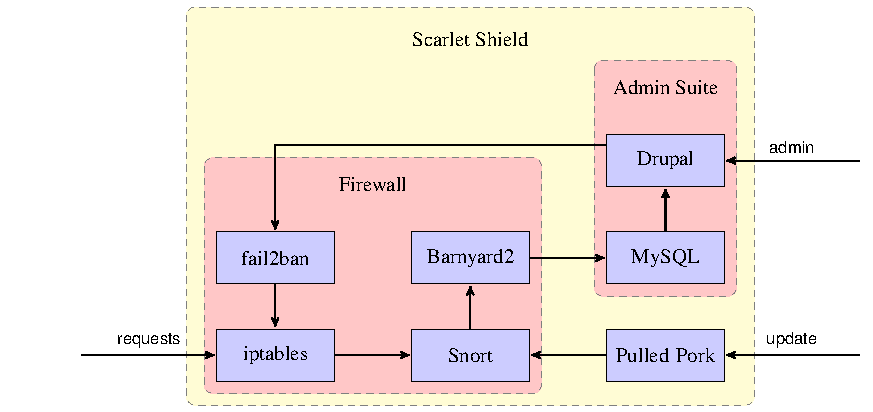
\includegraphics{./scarlet-shield-diagram2.pdf}
  \caption{The architecture of Scarletshield. Incoming packets are routed
  through iptables, where they may be blocked per iptables' rule-set; Snort receives
  the packets and inspects them for signatures of attacks; offending packets are 
  mirrored via Barnyard2 into a MySQL database; users can access the Administrator
  Suite provided by Scarletshield and hosted using Drupal in order to analyze
  attacks against the system; fail2ban automatically bans abusive foreign hosts. 
  Pulled Pork is used to automatically update Snort's classification rulesets
  for offending packet patterns.}
\end{figure}

Scarletshield was implemented behind a Ubuntu 12.04 LTS Server edition for
purposes of stability and universality.  In addition, the “LTS” acronym stands
for Long Term Support, a term coined by Canonical, the developers of Ubuntu,
that essentially means that they are supporting and supplying security updates
for the Ubuntu 12.04 LTS for five years from its release date.  Ubuntu 12.04 LTS was
released in April of 2012 (hence, it is version 12.04) and thus Scarletshield will
have a completely secure operating system until April 2017.  Note, however, that
most of the subsystem software components to be listed in this section are
cross-platform, and thus compatible with other contemporary Linux distros and
even modern Windows operating systems to an extent.  This speaks to the
scalability of the Scarletshield concept, which will be discussed in a later
chapter.

Specifically, here is a breakdown of each component that builds the full
software architecture behind Scarletshield, starting with Snort followed by each
successive in the diagram component:

\begin{enumerate}
\item Snort 2.9.X (2.9.3 is used for Scarletshield) -- A free and open source IDS
developed by Sourcefire, Inc. suited towards network intrusion prevention,
which is one of the core functions behind Scarletshield.  Snort works by creating a
separate, virtual and promiscuous (meaning that all packets received by
Snort’s separate interface gets directed to the central processing unit for
inspection) interface that copies traffic off of the network card as it is
received, enabling the simultaneous inspection of packets as they reach
their intended destination in a timely manner.  This means that
Scarletshield is able to inspect packets without creating any latency or
overhead experienced by clients actually intended to receive said packets,
since Snort is only inspecting carbon copies of said packets, instead of
the actual packets, as they pass through Scarletshield. To work effectively
and stay up to date with the latest updates, Snort utilizes a ruleset of
known and relevant exploits and employs pattern-matching to catch packets
suspected of malicious activity.  How is Snort kept up to date?  It uses
another critical component for updating known as Pulled Pork.
    
\item Pulled Pork (the Perl script is sometimes referred to in its concatenated
form, PulledPork) is not actual software, but an open source Perl script also by
Sourcefire, Inc. that incorporates rule updating and management that facilitates
the timely, monthly updating of the Snort IDS.
    
\item  Barnyard2 -- When Snort executes its packet inspection, and finds suspect
packets which  trigger a signature identifying a pattern of malicious activity,
it presents a number of logging options.  Out of its options, the most
lightweight and most efficient method of logging and consolidating these suspect
packets is via unified2 (u2) binary logging.  The optimal means of reading and
working with such logs is via an open source interpreter known as Barnyard2.
Taking the u2 logs, barnyard2 will continuously process data that is written
into them by the Snort IDS and output this data into readable data in a format
that is then readable by an administrator via a database.
   
\item MySQL -- A heavyweight, well-established, and open-source database management
system, we utilize MySQL to integrate all records of packets captured by the
Snort IDS and translated by the Barnyard2 interpreter.

\item Drupal/JavaScript -- We used the PHP-based Drupal CMS to build
scarletshield.rutgers.edu, our primary front-end for the presentation of our
data. While we originally intended to integrate the MySQL database of our
packets into Drupal directly, we actually found that utilizing javascript for
the presentation of this data was a far more presentable alternative.  This is
what facilitates administrators/users being able to view our data on a web
browser.

\item fail2ban -- Working in parallel with the Snort IDS, fail2ban is an IPS based
on Python that utilizes log inspection to facilitate the proactive blacklisting
of IP addresses that are the source of malicious activity, specifically brute
force attacks out-of-the-box, and interfaces with the built-in firewall on
modern Linux kernels managed by user space application, iptables, to drop
packets from aforementioned malicious activity sources.  By itself, it is unable
to protect against more sophisticated exploits and attacks such as distributed
denial-of-service.  When reinforced with an IDS such as Snort, however, and
integrated in our Scarletshield system, they can together log and stop a large
volume of known attacks.

\item iptables -- A user space application enabling management over the Linux kernel
firewall via a system of chains and rules.  The iptables name also refers to the
entire kernel-level subsystems that make up the Linux kernel.
   
\end{enumerate}


\chapter{Approach and Methodology}

As we are designing Scarletshield from scratch with a Ubuntu 12.04 LTS server,
there are several sections to our Approach and Methodology:

\begin{enumerate}
\itemsep0em
\item Design \& Approach
\item Employing Two-point Authentication over SSH
\item Set up of Snort and fail2ban
\end{enumerate}

\section{Approach}

To summarize the process in the previous chapter's system software architcture subsystem
breakdown -- \scarletshield takes all incoming packets and either accepts or drops them based
on iptables, which is built in to modern Linux \distros such as Ubuntu 12.04 LTS
automatically.  What makes \scarletshield unique is how we deploy an IDS and IPS
through Snort and Fail2ban.  Specifically, IDS mirrors all packets and analyzes
them for patterns (via Snort rules, which are updated every month over the
Internet) indicative of a potential threat, then logging threat signatures on a
database accessible to the administrator and analyzed for new, more strict
iptables rules banning offending IP addresses where necessary.  We utilize
fail2ban to detect obvious brute force, overflows, and exploits in the server
logs (/var/log/auth.log, etc.) to also automatically filter and block IP
addresses preventively, requiring no action from the administrator.

Thus, with the Snort IDS and fail2ban IPS working in concert with the
administrator and the kernel-level firewall managed via iptables, the 
Scarletshield approach accomplishes the following two critical objectives:

\begin{enumerate}
\item Implements a level of automation to immediately act against obvious threats requiring no action from the administrator.

\item Captures more ambiguous threats with the potential of attempted penetration 
and attacks against the Server and presents it to the administrator via a web-accessible 
front-end that gives the administrator an analysis enabling further policy control to help thwart potential threats. 

\end{enumerate}


\section{Employing Two-point Authentication over SSH}

Through our research as a group, we came to the conclusion that the safest way
to protect our SSH  server against brute forcing would be to change our SSH’s
port from 22 to create security through obscurity.  However, 
in order to gather the largest possible set of logged attack data,
we needed to present SSH on its standard port.
This led us to a different approach of setting up two-factor
authentication.  By utilizing Google’s ``Google Authenticator API'', 
in order to successfully
gain access to ScarletShield’s SSH server, one must first enter the correct
password and the unique TOTP security token, described by RFC6238 and generated by the
``Google Authenticator'' app, for the specific user trying to login.  This security
measure makes it impossible for a malicious user to gain login access through
brute fore.

\begin{figure}[h!]
\centering
  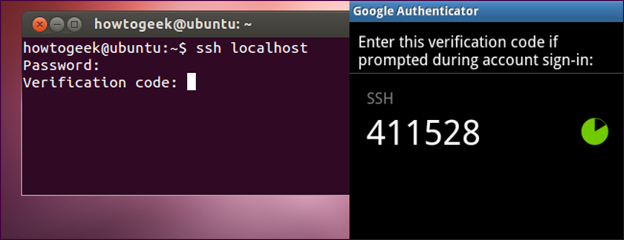
\includegraphics{./goodleauth.png}
  \caption{(Left) A prompt to enter a Google Authenticator verification
  code after typing in a password. (Right) Google Authenticator smart phone application
  generating a verification code.}
\end{figure}

\section{Installation}

Scarletshield covers the breadth of IPS and IDS by implementing both fail2ban
and Snort and interfacing the former with iptables, a user space application for
packet handling.  This not only enables the mobility for a network administrator
to easily be able to monitor incoming traffic and potential threats on a switch,
but also provides an automated mechanism via fail2ban to block obvious, trivial
threats such as brute force attacks and denial-of-service.

Fail2ban is a very simple installation in Ubuntu 12.04 LTS, since it is included
in the advanced packaging tool.  Using its internal mechanism known as ``jails'',
it essentially utilizes filters implemented based on obvious threats (brute
force over SSH, flooding over apache, etc.) and, over a user-set period of time
(default period is several minutes long), bans offending IP addresses for the
duration after it gets caught by Fail2ban via iptables directives packaged with
the program.

Snort is a larger beast with many different variations of configurations
available (types of relational databases used, logging mechanism, etc.); at the
very least, an administrator separately needs to acquire and install libdnet and
the Data Acquisition API \autocite{snort}.  In addition, an administrator must choose a
database and correctly install and configure its respective libraries and server
application.  Due to how fully featured it has become over the years, we chose
MySQL.

In our Ubuntu 12.04 LTS Server Edition and extensible to any Debian based
system, fail2ban is available via the built-in Advanced Packaging Tool (APT),
and can be installed practically instantaneously via the following command-line
directive:
\begin{minted}[frame=lines,framesep=2mm]{console}
    apt-get install fail2ban
\end{minted}
Due to how comprehensive the Snort IDS is and how it integrates with Pulledpork
and Barnyard2, there are several of steps to successfully deploying Snort,
Pulledpork, and Barnyard2 on Linux distributions, and thus the instructions
typically vary depending on the specific operating system involved.  Our
instructions is largely derived from the Snort Install Guide 2.9.3 for Ubuntu
Linux, and the process we took is as follows:

The Snort IDS has several of requirements, thus, we thoroughly utilized the
Advanced Packaging Tool that comes packaged in Ubuntu 12.04 LTS to install the
following programs via the following apt-get install directive:


\begin{minted}[linenos,numbersep=5pt,frame=lines,framesep=2mm]{console}
sudo apt-get install nmap, nbtscan, apache2, php5, php5-mysql, php5-gd,
    libpcap0.8-dev, libpcre3-dev, g++, bison, flex, libpcap-ruby, make,
    autoconf, libtool, mysql-server, libmysqlclient-dev
\end{minted}

Next, ensuring maximum security, we applied all software and distribution
updates as follows:
\begin{minted}[linenos,numbersep=5pt,frame=lines,framesep=2mm]{console}
sudo apt-get install update 
sudo apt-get install upgrade
\end{minted}
There are two more requirements for Snort that are unfortunately not available
through the Advanced Packaging Repository.  They are the Data Acquisition API
and libdnet.  These are available directly via the snort.org website and libdnet
google code repository, respectively, and we acquired and installed them as
follows: 
\begin{minted}[linenos,numbersep=5pt,frame=lines,framesep=2mm]{console}
sudo wget http://www.snort.org/downloads/1806 -O daq.tar.gz 
sudo tar xzvf daq.tar.gz 
cd libdnet 
sudo ./configure 
sudo make 
sudo make install
\end{minted}
The above commands round out the Data Acquisition API installation. We moved on
to installing libdnet as follows: 
\begin{minted}[linenos,numbersep=5pt,frame=lines,framesep=2mm]{console}
sudo wget http://libdnet.googlecode.com/files/libdnet-1.12.tgz -O libdnet.tar.gz 
sudo tar xzvf libdnet.tar.gz 
cd daq 
sudo ./configure 
sudo make 
sudo make install     
sudo ln -s /usr/local/lib/libdnet.1.0.1 /usr/lib/libdnet.1
\end{minted}
Now all the required software components are installed and up-to-date, we moved
on to installing Snort 2.9.3 directly!
\begin{minted}[linenos,numbersep=5pt,frame=lines,framesep=2mm]{console}
sudo wget http://www.snort.org/downloads/1814 -O snort.tar.gz 
sudo tar xzvf snort.tar.gz 
cd snort 
sudo ./configure --prefix=/usr/local/snort --enable- sourcefire 
sudo make 
sudo make install 
sudo mkdir /var/log/snort    
sudo mkdir /var/snort 
sudo groupadd snort 
sudo useradd -g snort snort 
sudo chown snort:snort /var/log/snort
\end{minted}
At this point, Snort needs a rule set. This is when Pulledpork comes to play.
Pulledpork, being perl-based, has additional software requirements, which are
also thankfully available via APT as follows: 
\begin{minted}[linenos,numbersep=5pt,frame=lines,framesep=2mm]{console}
apt-get install libcrypt-ssleay-perl liblwp-useragent-determined-perl -y
\end{minted}
Pulledpork was retrieved and installed as follows into the Snort install folder:
\begin{minted}[linenos,numbersep=5pt,frame=lines,framesep=2mm]{console}
cd /usr/local/snort 
wget https://pulledpork.google.com/files/pulledpork-0.6.1.tar.gz 
tar -xzvf pulledpork-0.6.1.tar.gz 
cd pulledpork-0.6.1 
mv pulledpork.pl /usr/local/bin/
\end{minted}
From this point forward, there are several of fine-tuned configurations that we
made. Specifically, we created an /etc/snort directory and changed into it,
inserting a configuration file which we also have available on our web server as
follows: 
\begin{minted}[linenos,numbersep=5pt,frame=lines,framesep=2mm]{console}
sudo mkdir /etc/snort 
cd /etc/snort 
wget http://scarletshield.rutgers.edu/snort.conf     
chmod og-wr snort.conf 
\end{minted}
The last
command above ensured maximum security by preventing unauthorized users from
prying into or possibly editing your snort configuration.  Next, we created a
rules folder and populated it as follows:     
\begin{minted}[linenos,numbersep=5pt,frame=lines,framesep=2mm]{console}
sudo mkdir rules     
wget http://scarletshield.rutgers.edu/snort.rules 
\end{minted}
A pulledpork configuration
directory was downloaded and unpacked via the following configuration files:
\begin{minted}[linenos,numbersep=5pt,frame=lines,framesep=2mm]{console}
sudo mkdir /etc/pulledpork     
cd /etc/pulledpork/ 
sudo wget http://scarletshield.rutgers.edu/pulledpork.tar.gz 
sudo tar xzvf pulledpork.tar.gz 
\end{minted}
Updates via our new Pulledpork configuration are asserted as
follows: 
\begin{minted}[linenos,numbersep=5pt,frame=lines,framesep=2mm]{console}
pulledpork.pl -c /etc/pulledpork.conf	
\end{minted}
For our last software subsystem component, we installed barnyard2 as follows:
\begin{minted}[linenos,numbersep=5pt,frame=lines,framesep=2mm]{console}
wget https://nodeload.github.com/firnsy/barnyard2/tarball/master 
    -O barnyard2-2.10.tar.gz 
sudo tar zxvf barnyard2-2.10.tar.gz 
cd firnsy-barnyard2* 
sudo autoreconf -fvi -I ./m4 
sudo ./configure --with-mysql --with-mysql-libraries=/usr/lib/i386-linux-gnu 
sudo make 
sudo make install 
sudo cp etc/barnyard2.conf /usr/local/snort/etc 
sudo mkdir /var/log/barnyard2 
sudo chmod 666 /var/log/barnyard2 
sudo touch /var/log/snort/barnyard2.waldo 
sudo chown snort.snort /var/log/snort/barnyard2.waldo
\end{minted}
The last components of the installation are with regards to the database, which
we generated as follows:     
\begin{minted}[linenos,numbersep=5pt,frame=lines,framesep=2mm]{console}
echo “create database snort;” | mysql -u root -p
mysql -u root -p -D snort < ./schemas/create\_mysql     
echo “grant create,insert, select, delete, update on snort.* to 
    snort@localhost identified by ‘OURSECRETPASSWORD’” | mysql -u root -p
\end{minted}
Finally, we set up the network cards:     
\begin{minted}[linenos,numbersep=5pt,frame=lines,framesep=2mm]{console}
sudo vi /etc/network/interfaces
\end{minted}
In the vi text editor, we added the following lines to add the mirrored,
promiscuous interface that Snort would be utilizing:
     
\begin{minted}[linenos,numbersep=5pt,frame=lines,framesep=2mm]{console}
auto eth1 iface eth1
inet manual         
    up ifconfig \$IFACE 0.0.0.0 up         
    up ip link set \$IFACE promisc on         
    down ip link set \$IFACE promisc off         
    down ifconfig \$IFACE down
\end{minted}

This is the rigorous installation process we undertook for Scarletshield.
Having installed the entire back-end, we can now continue on to the
Administration Suite and Features.


Once Snort and the database being used are installed, the user must then acquire
and/or update the Snort rule-set, which is essentially how Snort is able to parse
and detect threats within the headers and contents of packets entering the
machine.  We chose ``Pulled Pork'', as it is the most reliable Snort rule management
application, recommended by the creators of Snort themselves.  Finally, the
administrator must interface Snort with the MySQL database.  As of Snort
2.9.3.0, the latest stable version available for Ubuntu 12.04 LTS, it is
required to install the application ``Barnyard2'' for a Snort daemon to record
information into the MySQL database created by a user.

\chapter{Administration Suite \& Features}

\section{Web Front-end Integration}


Scarletshield features a web frontend utilizing a simple but powerful Drupal
Content Management System (CMS).  In addition, several PHP scripts are
utilized to help analyze and serve the Snort MySQL database.

Scarletshield has three powerful tools for a user that wishes to learn more
about the offending attacks against their server. These three tools, the ``Attack
History'', ``Analytics'' and ``Heatmap'' pages, all come comprise
Scarletshield Suite. Each tool features a different way for the user to view
the logs stored by Scarletshield. The link for the Scarletshield Suite is
\url{http://scarletshield.rutgers.edu/suite}.\footnote{Note that the Scarletshield Suite was
written for the Chrome browser, and some small details will not work on other
browsers.}

\begin{figure}[bth]
\centering
  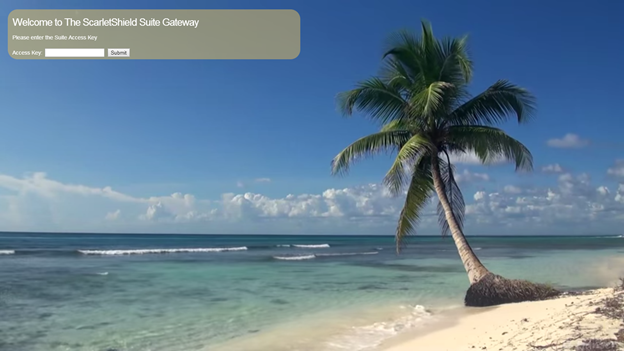
\includegraphics[height=8cm]{./login.png}
  \caption{The Scarletshield Suite login page.}
\end{figure}

When a user tries to access any page of the suite, a JavaScript function runs to
see if the user has an active login cookie with the correct password (the
password is ``scarlet'').  If the user does not have this cookie, they are
redirected to the suite login page seen below.


The login page makes use of two JQuery packages.  The first package,
``Tubular'', allows a streamed video to be the page background.  The other
package, ``Toastr'', makes use of JavaScript’s non-blocking
architecture.  Toastr is responsible for all asynchronous pop-up alerts.  These
can be seen at page load, and when the access key form's ``Submit'' button is
pressed. Upon entering the correct password, the login cookie is generated and
the user is then brought to the ``Attack History'' page. When first accessing this
page, a loading animation is shown, while the back-end queries data from the MySql
database containing all Snort logs. As a large dataset is loaded from the
server, a screen similar to the one shown below is displayed.

\section{Analytics}

\begin{figure}[b!]
\centering
  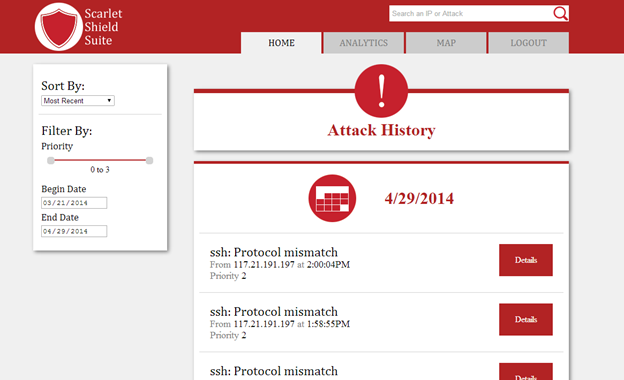
\includegraphics[height=8cm]{./history.png}
  \caption{The Scarletshield Suite Attack History page.}
\end{figure}

Immediately upon visiting the page, the user is given access to all the data
that Snort has logged; the data are logically and visually organized and to
maximize presentability. (For comparison, an early implementation of this
page can be seen here: \url{http://scarletshield.rutgers.edu/demo/last100.php }.) 
Each log is grouped by date and contains information
about the type of attack, the IP address it was originated from, the time it
occurred and the priority of the attack (on a range from 0 to 3 with 0 being
highest priority). If the user presses the ``Details'' button, extra information,
such as the destination IP address (which may not be static if the server has
more than one IP address), the ID number of the occurrence, and approximate
location of the attack are expanded.


\begin{figure}[t!]
\centering
  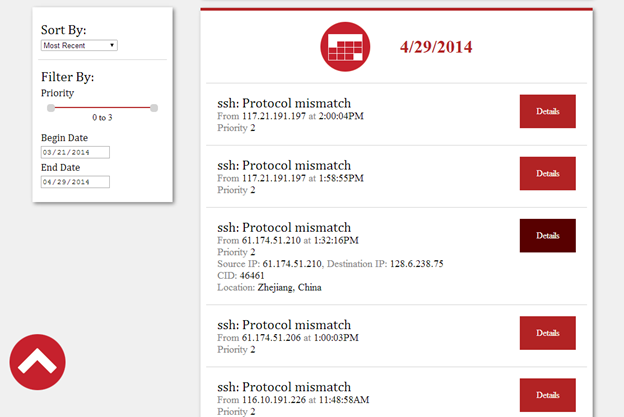
\includegraphics[height=8cm]{./historydet.png}
  \caption{The Scarletshield Suite Attack History page, with an expanded
  description of the details of an attack originating from China.}
\end{figure}

On the top left hand sides of the page, several tools allow the user advanced
filtering capabilities. Logs can be sorted by date (oldest or newest) and
priority (lowest first or highest first), and the search bar at the top can be
used to only show information that either contains the IP address we search or
show attacks that match the string that was searched. This is incredibly
convenient because manually querying for signatures in MySQL (which involves
several tedious SQL joins) would be a time-consuming task for an administrator,
and by having it presented via an admin-accessible private frontend, not only
could administrators react quicker, but even less-skilled users could discover
and report an ongoing attack.

\begin{figure}[b!]
\centering
  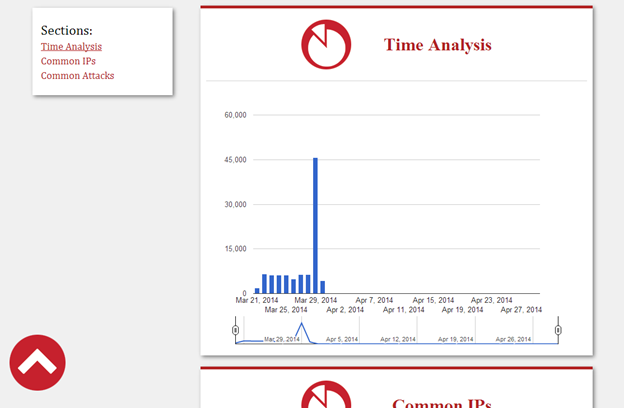
\includegraphics[height=8cm]{./timeanalysis.png}
  \caption{A chart of the rate of attacks over a certain interval. Users
  can use the slider at the bottom of the chart to analyze attacks over
  arbitrary intervals.}
\end{figure}

The Analytics page has three sections, as noted on the sidebar: the “Time
Analysis”, “Common IP’s”, and “Common Attacks”. The Time Analysis section is
simply a chart that shows a chart with the number of attacks that the server has
undergone each day. This chart has a slider to focus on specific time intervals,
and as one can see from the entire view, this is necessary because one single
day may be so active that it dwarfs other days’ activity.


\begin{figure*}[h]
\centering
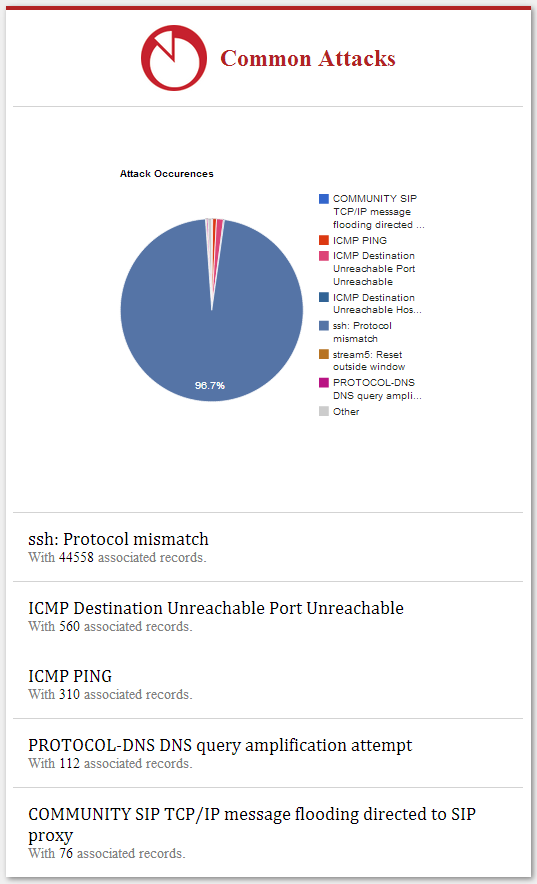
\includegraphics[width=0.45\textwidth]{attackpie.png}\hfill
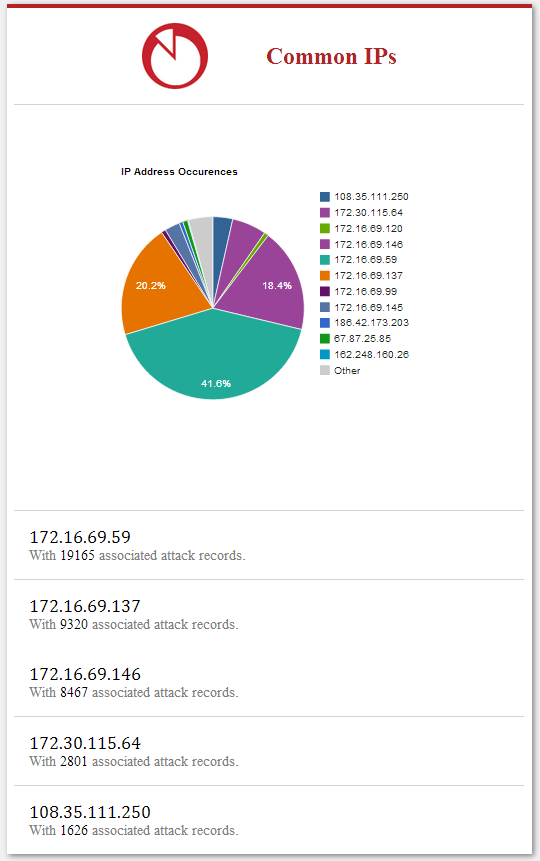
\includegraphics[width=0.45\textwidth]{ippie.png}
\caption{Pie charts featuring prominent attack varieties and IP addresses.}
\end{figure*}

The last page in the Scarletshield Suite is the Heatmap page. Essentially,
Scarlet Shield processes IP addresses from all logged attack patterns and places
it on a Google Map heatmap, so that the user may be able to geographically
backtrace signatures.  In certain configurations, the heatmap would be useful to
backtrace potential ongoing threats and attacks, such as DoS attacks within
certain windows.  This would also help administrators make informed decisions
for creating temporary iptables rules for banning certain offending subnet
servers for the duration of an ongoing threat. An example of the heatmap is
shown below. 

\begin{figure}[h!]
\centering
  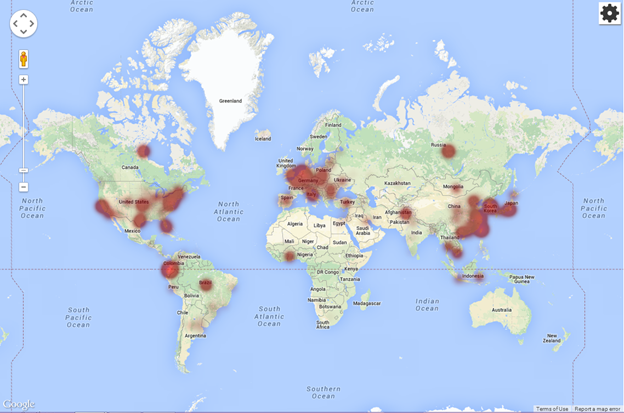
\includegraphics[height=8cm]{./heatmap.png}
  \caption{A geographic world map with red intensity markers indicating
  the presence of attack vectors from a geographic region, identified by IP address.}
\end{figure}

\section{Response Options}

The final portion enabling Scarletshield to cover the full spectrum of network
defense is enabling the network administrator to utilize the frontend for
analysis and decision-making options.  Essentially, the an administrator should
be able to take the Snort records, make an analysis, and decide the action
(whether to throttle or drop all packets altogether from a suspicious IP
address) to take to ensure network security.

Due to time constraints, this feature was not integrated into the administrator
suite, although the capability is already inherently present because of the
inclusion of fail2ban. Future work could easily incorporate the addition of such
an administrator response suite.

\chapter{Conclusion}


\section{Cost/Sustainability Analysis and Scalability}

In spite of existing in an aged Microway rackmount server, the primary component 
necessary for utilizing Scarletshield on a network gateway is the Network Card.  While a 
dedicated rackmount server is a costly investment, much of the hardware that 
Scarletshield actually runs off of is dated and can be purchased for very 
cheap prices off the shelf.  One of its most important elements, a NetXtreme 
BCM5721 Gigabit Ethernet PCI Express card, actually goes for \$15-\$70 (depending 
on where you look, and on whether it is used or refurbished). 

Scarletshield in its current manifestation operates off of a Microway rackmount 
server.  An equivalent, but modern-day, rackmount server would range between 
\$2,000-\$5,000, which would be a large investment. 
A modern rackmount server running an operating system and network security suite
comparable to Scarletshield would be able to scale to meet the demands of
thousands and possibly even millions of clients and internal gateway server
connections.  To this end, however, the network cards would need to be far more
powerful, possibly in the territory of 10Gbps+.  Network cards that powerful
could be hundreds to thousands of dollars or additional cost, but would only be
necessary for the case of an ISP or server farm scale of operations.      

It is
important to note that Scarletshield does not require dedicated hardware to the
aforementioned extent, however.  Scarletshield could be installed into
refurbished desktops with an extra network card and still be serviceable; this
would actually be a very useful and cheap method of creating a homemade network
security suite to use for a small business or home.  An equivalent desktop
computer with the hardware specifications that our dated Microway rackmount
server brings forth would likely only be a few hundred dollars.

All the
software utilized is free and, for the most part, open source.  Thus, this is
what makes the Scarletshield approach so desirable.  As opposed to spending
hundreds to thousands of dollars on a hardware-based intrusion detection and
prevention system, a savvy network or system administrator would be able to
implement their own and be able to extend their server for functions other than
dedicated intrusion detection or intrusion prevention.  Scarletshield, for
example, hosts its own web server from inside the server.       

What makes
Scarletshield so cost-effective is that the server is not necessarily restricted
to the network security suite.  You would be able to host additional web sites
and databases on your gateway and maximize utility.  The tradeoff would be that,
being tied to the same server as the IDS/IPS, downtime may be somewhat higher
due to the maintenance requirements of a network security system warranting
updates and upgrades often to remain effective.  Nevertheless, reboots and other
functions of maintenance actually requiring downtime is not exclusive to the
network security system alone; thus, a network or system administrator would not
experience grief exclusive to integrating the IDS/IPS into a production server.


In summary, while Scarletshield in its current state can handle traffic from the
scale of hundreds to thousands of connections, the core software architecture
can actually be scaled down for a small business or home application by being
installed in cheaper hardware and scaled up to handle thousands to millions of
connections by being installed in enterprise-grade hardware.  Utility with
Scarletshield is maximized with pitted against a hardware IDS/IPS in that
Scarletshield can double as a production server.  Overall, that makes
Scarletshield both cost-effective, sustainable, and scalable in the long-term!


\section{Future Work}

Although Scarletshield is already operational on a server within Rutgers
Engineering, additional work is necessary to integrate it into private subnets
and to give it world-wide-web scale. More robustness and failover capabilities
are needed in order to communicate certain threats that may be large-scale, and
which would otherwise disrupt significant cybersecurity infrastructure. This
also requires fine tuning Scarletshield’s frontend capabilities and adding more
analysis tools and automation techniques to streamline the threat-analysis and
threat-prevention workflow presented to the network administrator.  Further
integration of the subcomponents of Scarletshield will solidify its versatility,
relevance, and overall strength.  By successfully implementing a fully-featured
frontend for monitoring and reacting to threats, we will maximize the potential
of Scarletshield to be deployable to both private switches and enterprise-level
networks.

Primarily, this entails better integrating current monitoring scripts with
Drupal.

Moving forward we envision multiple ScarletShield deployments being used to
protect a multitude of systems simultaneously.  With this in mind we plan on
creating a global set of black lists and logs that all deployments can
access and update.  Maintaining global lists would allow each individual
deployment of ScarletShield to share collective knowledge. If one instance
of ScarletShield is attacked, another deployment can preemptively block the
attacker instead of waiting to be attacked itself.

Also, our scripts will allow administrators the option to take action on
addresses logged with signatures, along with varying degrees of reaction
steps they may be able to take (functionality to throttle or ban IPs
altogether, for example), such that Scarletshield will give full control to
the network administrator.

Additionally, we will be working on a way to replicate the Scarletshield
build; this will most likely be accomplished by presenting a ISO image that
can be installed in managed switch servers.

\section{Summary and Concluding Remarks}

During this semester, we achieved the following goals:

\begin{enumerate}
\item Build from scratch a specialized Ubutnu 12.04 LTS Server Edition-based
 network security system integrating the Snort IDS and fail2ban IPS to interface
  with its kernel firewall via iptables to automatically log and potential threats
   and drop all packets from packet sources confirmed to be malicious.
   
\item Integrate the IDS and IPS into a specialized front-end intended to maximize 
the analytical options available to system and network administrators enabling them 
to make quick and well-informed decisions on their network security policies flexibly 
depending on the type of traffic that Snort has been capturing. 
\end{enumerate}

%\begin{enumerate}
%\item Deployed a Ubuntu 12.04 LTS server with Apache, MySQL, Php, Drupal, Snort,
%		Pulled Pork, Barnyard2, fail2ban, and integrated them with iptables
%\item Configured Snort to update via Pulled Pork and to log to MySQL via Barnyard2
%\item Established initial rules and filters for Snort and Fail2ban
%\item Utilized PHP scripts to build monitoring and analysis suite into Drupal
%\item Provided dynamic and user-friendly analytics charting and mapping tools
%\end{enumerate}

Our work in integrating the Snort IDS, fail2ban IPS, and iptables within the 
\url{http://scarletshield.rutgers.edu} web server has culminated in the final 
development and release of a robust frontend, the Scarletshield Suite, which is
available via \url{http://scarletshield.rutgers.edu/suite} using the password 
“scarlet”. Our overall framework presents a great proof-of-concept for an open-source
solution for network security that can be applicable to small-time enterprises and
individuals who would not prefer to invest in a proprietary or commercial IDS or IPS. 

After a little over a month of being online, Scarletshield has caught over 100,000 
suspicious packets suspected of attempting penetration or exploitation of our server.
(Exemplifying how effective our work in Scarletshield has been this semester, 
Rutgers Engineering Computing Services (ECS) has tasked system administrator 
Val A. Red with replicating the Scarletshield Suite for internal use to monitor 
wireless access point gateways.)

We created a lightweight system of integrated network security via a front-end suite 
presenting the capabilities of both the Snort IDS and the fail2ban IPS in a way that
maximizes automation and ease-of-use for the network and system administrator.  
Nevertheless, there are some features that could be added to make Scarletshield even more robust.  
Specifically, a distributed version of the threat analysis database and iptables could have 
been developed such that other networks beyond our own can share information on threat sources 
and types of attacks, being a more consolidated solution for types of threats such as DDoS. 
The scale of that type of feature, however, could warrant its own design project entirely!  
With regards to the work we accomplished over the semester, there is great significance in the
proof-of-concept Scarletshield represents. As opposed to utilizing a completely security-based
Linux distribution such as how Security Onion presents itself, Scarletshield presents a subsystem
of capabilities that can be appended to an existing gateway or DHCP server, such as how
Scarletshield is going to be introduced to our wireless access point gateways.  
That alone speaks to success and confidence built in our final Capstone Design product.

Scarletshield is a comprehensive proof-of-concept network security solution suite that has 
been proven to capture and eliminate potential threats from around the globe 24/7! 

\section{Contribution Breakdown}

Scarletshield, an ambitious endeavor to present a large-scale network solution
suite,  was conceived and developed by a group of five undergraduate senior
Electrical and Computer Engineering Students of Rutgers University’s School of
Engineering.  They are Jeff Adler, Eric Cuiffo, Parth Desai, Jeff Rabinowitz,
and Val Red.  Due to the grand scale and major objectives of the projects, heavy
contributions were made by each and every member. Thus, it can be estimated that
each member had a specialized role that actually created a nice, even split of
fifths such that without the fifth contributed by each member, the whole of
Scarletshield would have failed. The contributions are broken down as follows,
in the same alphabetical order:

Jeff Adler -- Committed work on the extra-secure methodologies employed in
Scarletshield, such as the two-point Google Authentication implemented for our
Secure Shell (SSH) access, the Site Access Key authentication greeter for the
administrative Scarletshield Suite.

Eric Cuiffo -- Led the effort for an expansive, robust front-end for the
Scarletshield based on javascript and jQuery. The suite scripts he predominantly
led the effort on, also to be presented in the Appendix section, were
instrumental for the front-end presentation of the Scarletshield Suite.  He also
had the greatest contribution to the Scarletshield Heat Map, which takes all
potential threat connection sources and actually interpolates geolocation data
into a map of the world!

Parth Desai -- His experience with PHP and MySQL enabled our early, prototype
work on the Scarletshield Suite backend to run smoothly.  Specifically drafting
how we would translate the database to our web frontend, Parth Desai was
instrumental in the integration of the backend database and the frontend suite
via queries.

Jeff Rabinowitz -- Resident expert on relational databases and LaTeX, Jeff
Rabinowitz contributed insight that ensured that not only our queries were as
efficient as possible, but that this report was optimally presentable.  His
ability to work with databases specifically ensured that the Scarletshield Suite
was a success in enabling real-time analysis of the data parsed by Snort.

Val A. Red -- A system administrator by trade, Val Red implemented the
installation phase of the backend, ensuring Snort and fail2ban worked seamlessly
and did not break the Ubuntu 12.04 LTS installation or Scarletshield’s Microway
Server altogether.  Specifically, his rigorous configurations (.conf files will
also be in the appendix) and fine-tuning maximized performance and allowed the
Scarletshield Suite to work seamlessly by ensuring no errors or failures would
occur in the extensive back-end, maximizing speed and efficiency between Snort,
fail2ban, and the entire Scarletshield system.

All group members made great, synergistic contributions such that the whole of
Scarletshield summed together amounted to a design far greater than its parts.
In addition, there was a lot of overlap and cross-specializations such that in
addition to the aforementioned specialized contributions, practically every part
of the final product was a result of all team members working together. We are
proud of our work on Scarletshield, and have learned a great deal about network
security and systems programming overall in building it!



}
\printbibliography

\end{document}